\subsection{Ondas estacionárias de som: geração de harmônicos em
função do comprimento L}

O terceiro experimento consiste em analisar a geração de harmônicos em função da variação do comprimento L da coluna de ar. Por se tratar da geração de ondas estacionárias de som, a prática em questão foi realizado no mesmo dispositivo descrito no tópico anterior. Entretanto, a frequência de excitação f produzida pelo gerador é fixada e os harmônicos serão gerados variando a posição do pistão móvel de modo a obter valores diferentes para o comprimento da coluna de ar.

\begin{figure}[H]
  \centering
  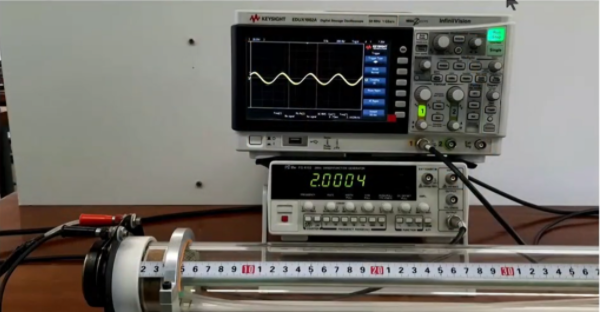
\includegraphics[scale=0.9]{images/frequencia f.png}
  \caption{ Registro da frequência f fixada para o experimento.}
\end{figure}

Com base na relação da velocidade de propagação da onda progressiva ($v = \frac{\lambda}{t} = \lambda \cdot f$), como a frequência \textit{f} está fixa, o comprimento de onda $\lambda$ deve ser constante. Portanto, da equação para obter uma onda estacionária ($n \cdot \frac{\lambda_n}{2} = L$), o comprimento do tubo somente assumirá valores $L_n$ dados pela seguinte relação:

\[ L_n = n \cdot \frac{\lambda}{2}\]

Inicialmente, a frequência f utilizada é fixada em um valor da ordem de 2 kHz. Após isso, desloca-se os valores de $L_n$ de modo a obter ondas de pressão com intensidade máxima, correspondendo a condições de onda estacionária. O pistão é posicionado próximo ao alto-falante para ter certeza que o modo fundamental será detectado.

A partir dos sucessivos harmônicos n, registra-se os valores de $L_n$ correspondentes para, então, construir uma tabela relacionando ambos os dados. Uma terceira coluna é adicionado a tabela para representar as diferenças entre valores sucessivos $L_{n+1}-L_n$.

Dessa forma, a partir dos dados obtidos, o valor mais provável de $\lambda$ é determinado com sua respectiva incerteza. Com o valor do comprimento de onda ($\lambda$), calcula-se a velocidade do som no ar, com sua respectiva incerteza, com base na equação da onda progressiva já citada anteriormente. Esse valor calculado será comparado com os dados obtidos na prática anterior e com os valores de referência para, então, concluir se o experimento obteve resultados satisfatórios.
